



\section{Textual Analysis in Natural Language Software Artifacts}
\label{cp2:text-in-se}



In this section, we detail empirical studies investigating 
textual data in natural language software artifacts. 
Such textual data is  rich in semantic information~\cite{dekhtyar2004} 
and we provide and overview of seminal work 
investigating lexical, syntactic, and semantic aspects of the text 
in natural language software artifacts.




Initial insights about the text of a natural language artifact might be learned focusing on 
the characters or tokens in the text.
This lexical analysis~\cite{jurafsky2014speech} might be used to identify common or unique words 
used in an artifact as well as common words that often appear together  in the text. In software engineering research, Bacchelli et al. used lexical analysis to study how developers describe class elements
in nearly 80,000 emails of an Open Source System~\cite{bacchelli2009}.
Their analysis suggested that lexical terms could be 
used as a mean of automatically linking information in development emails to 
the project's source code.







Syntactic analysis concerns the  elements in the text 
and the grammatical relationships between them~\cite{jurafsky2014speech}. 
Part-of-speech tagging and dependency parsing are common applications of syntactic analysis,
where they identify the nouns, verbs, pronouns, and other elements in the text 
and how these elements relate, respectively. 
As an example of a syntactic analysis study in natural language software artifacts, 
Ko and colleagues identified regularities in the syntactic structure of the text 
of nearly 200,000 bug report titles~\cite{Ko2006}, suggesting that these 
regularities could be used for the automatic identification 
of information in bug reports. 

%  For example, Figure~\ref{fig:syntactic-analysis} shows the
%  Stanford CoreNLP~\cite{CoreNLP} syntactic analysis for a sentence 
%  about the file system:  `\textit{you can use io.StringIO}'.



% \medskip
% \begin{figure}[h!]
%     \centering
%     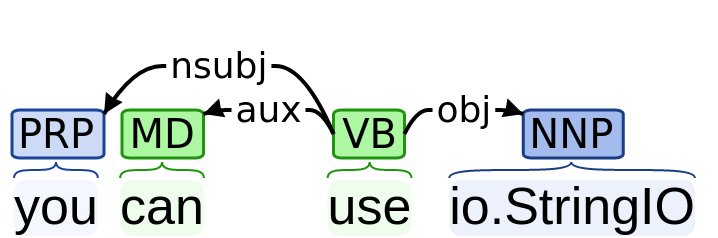
\includegraphics[width=0.40\textwidth]{cp2/textual-analysis.png}
%     \caption{Example of syntactic analysis}
%     \label{fig:syntactic-analysis}
% \end{figure}







Even sentences with similar terms or similar syntactic structure might convey different information
and software engineering researchers have also investigated the meaning of the text in natural language software artifacts. 
These studies consider the semantic analysis of the text and most of the existing 
work has focused on proposing \textit{taxonomies} to explain the type of information 
available in certain kinds of natural language artifacts~\cite{Maalej2013, Arya2019}. 
For example, Di Sorbo et al. have found that 
text in development mailing lists can be classified according to the developers' intentions (e.g., feature request, solution proposal, etc.)~\cite{Sorbo2015},
suggesting that one can automate this classification to assist developers in finding 
certain types of information.
% Other examples include Maalej and Robillard's taxonomy of patterns of knowledge in API documentation
% or Arya et al. analysis of information types in Open Source issues~\cite{Arya2019}.





Our thesis contributes to the body of empirical studies that investigate natural language 
text by characterizing common semantic cues across the text 
of different kinds of artifact that developers 
deemed relevant to a software task (Chapter~\ref{ch:characterizing}).







% This section details empirical studies analyzing different aspects associated with 
%  natural language software artifacts.






% Early studies on textual analysis in software engineering often focused on program comprehension 
% and the text in the source code~\cite{Woodfield1981, maletic2002},
% but 
% Researchers have long recognized 
% that natural language artifacts 
% are rich in semantic information
% and that 
% better understanding these artifacts
% would lead to improved software~\cite{dekhtyar2004}.






% These studies have helped
% software engineering researchers make more informed decisions 
% on the design of automated tools 
% that identify and extract text from these artifacts---detailed further in this chapter. 




% The empirical analysis provided by these studies 
% has 
% deepened software engineering researchers' knowledge of the type of information available 
% in natural language artifacts 






% Bird at al. used it to investigate social aspects in development mailing lists~\cite{bird2006}. 
% They inspected nearly 102,000 messages on the Apache HTTP Server development lists
%  to find that character editing algorithms~\cite{levenshtein1966}, 
%  helped in unmasking developers' aliases, which helped investigating email 
%  exchange patterns of the key contributors of the project.


% .
% They have sampled 100 emails and identified that text for feature requests 
% often contain expressions in the form of suggestions
% (e.g., `\textit{we should add a new button}'), whereas solution proposals 
% are often expressed in the form of attempts (e.g., `\textit{let's try a new method to compute cost}')





% With regards to meta-data 




% \clearpage


% Several other studies have 
% investigated the meta-data available in
% natural language software artifacts. 
% % In Section~\ref{cp1:example},
% % we have presented an example of meta-data in a Stack Overflow post,
% %  other examples include fields in a bug report~\cite{Davies2014, Breu2010},
% % or tags and labels in GitHub projects~\cite{prana2019}.
% These studies often focus on 
% the frequency with which
% meta-data is available~\cite{Davies2014, bettenburg2008makes, uddin2015},
%  how up-to-date it is~\cite{ahmad2018, dig2006, shi2011}, 
%  and the perils of relying on meta-data for information extraction purposes.
% For example, Zhang et al. has shown that 
% certain comments on Stack Overflow are equally or more informative 
% that the information found in an accepted answer~\cite{zhang2019so}.


% has led software engineering researchers to 
% make more informed decisions on when to use meta-data 
% and how it can assist in the extraction of useful information from natural language 
% artifacts.
% For example, Wang et al. 


% found that 

% the number of votes 
% an answer has on Stack Overflow is 
% equally or more important than 


% ~\cite{wang2018}



% ~\cite{wang2018}









% Findings from these studies led 
% software engineering researchers to discuss the promises and perils of 
% using an artifact's meta-data~\cite{kalliamvakou2014, ahmad2018}.
% For example, an accepted answer on Stack Overflow 
% might not be the correct answer~\cite{wang2018}
% and 
% valuable information exists in elements not
% associated with any meta-data~\cite{zhang2019so},
% which we discussed as part of our 
% scenario about finding information about Android notifications (Section~\ref{cp1:example}).